\subsection{Implementation Plan}
The TrackMe system will be implemented component by component, prioritizing the development of the most critical ones. Another key element on which the order of the implementation is decided is the level of dependency between components. This means that if multiple components depend on a single one then the development of the latter is prioritized upon the others, this way we can start integrating components as soon as they get developed and tested. Also it is considered good practice to concentrate first on the model part of the system, then to concentrate on the controller and at last on the view. For the previous reasons a Top-Down development approach has been selected.
\medbreak
\noindent
The following tree contains components as nodes and it is useful for describing the order of implementation from top to bottom following this rule: a node is implemented before its children. Therefore, the plan starts implementing the Database and the WebServer components in parallel.

\begin{figure}[H]
\centering
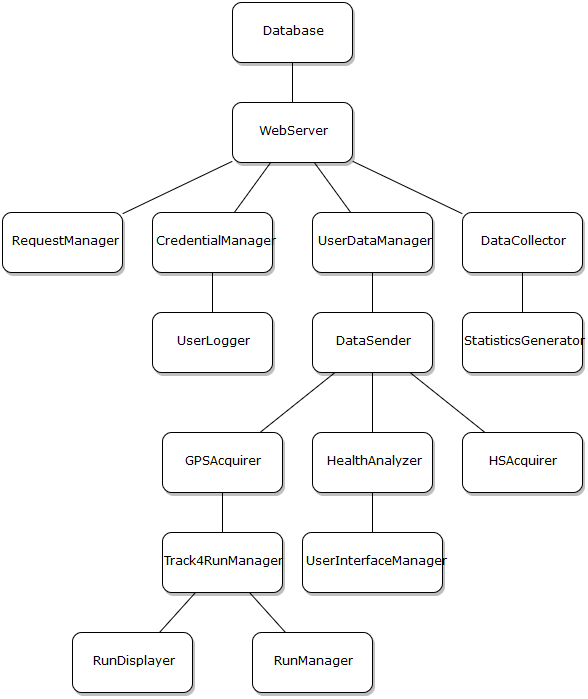
\includegraphics[scale=0.6]{Images/ImplementationPlan.png}
\caption{Implementation Tree}
\end{figure}

\noindent
One of the first components that will be implemented is the Database due to the fact that almost every component of the system will exploit Database's features, also it is one of the most critical parts of the system, if it fails then all our system will fail, and lastly, it forms the model of our system.
\medbreak
\noindent
The other component that will be implemented in parallel to the Database is the WebServer: it is one of the most critical element of our system as well, due to the fact that the third parties and the users will exploit this component to carry out every functionality that TrackMe offers.
\medbreak
\noindent
Then the components belonging to the second level of the tree will be developed since they form a big part of the business logic of our system and most of them manage information requests.
\medbreak
\noindent
As soon as the DataSender is completed, GPSAcquirer and HSAcquirer will be developed, since they interact directly with DataSender in order to store the retrieved data into the Database (already developed in the previous step). Then, once HSAcquirer is completed, the last two components of AutomatedSOS will be developed, starting with HealthAnalyzer, since it contains part of the logic of our system (in order to have faster reaction time), moreover, this component performs a critical functionality: calling an ambulance whenever necessary. Finally, the last component of this branch to be developed will be UserIntercationManager.

\subsection{Integration and Test Plan}
Every component of the system must be subjected to Unit Testing during its development in order to identify as soon as possible any problem within the component. This way, before actually preceding to any Integration Test, we are pretty sure that all components work well in isolation.
\medbreak
\noindent
As said in the previous subsection, the Integration Plan will also follow a Top-Down approach. More precisely, an \textit{Incremental Integration and Testing} approach is taken, since it couples really well with the dependency priority implementation order. This way, as soon as components that depend on others are released, they can be integrated and tested immediately, allowing us to discover integration problems as soon as possible.

\subsubsection{Integration Diagrams}
The following diagrams show the components to which the element just developed and already subjected to Unit Test is integrated with. The element just created is represented by a blue square, the grey ones on the upper lever represent already developed and unit tested components, while the grey ones on the same level represent components that could or could not be already developed and unit tested. In these diagrams, if there are more than one grey square, it does not mean that all the showed elements are integrated all together, but it means that they will be integrated just one by one, coupled with the one just developed or that will be developed soon.

\begin{figure}[H]
\centering
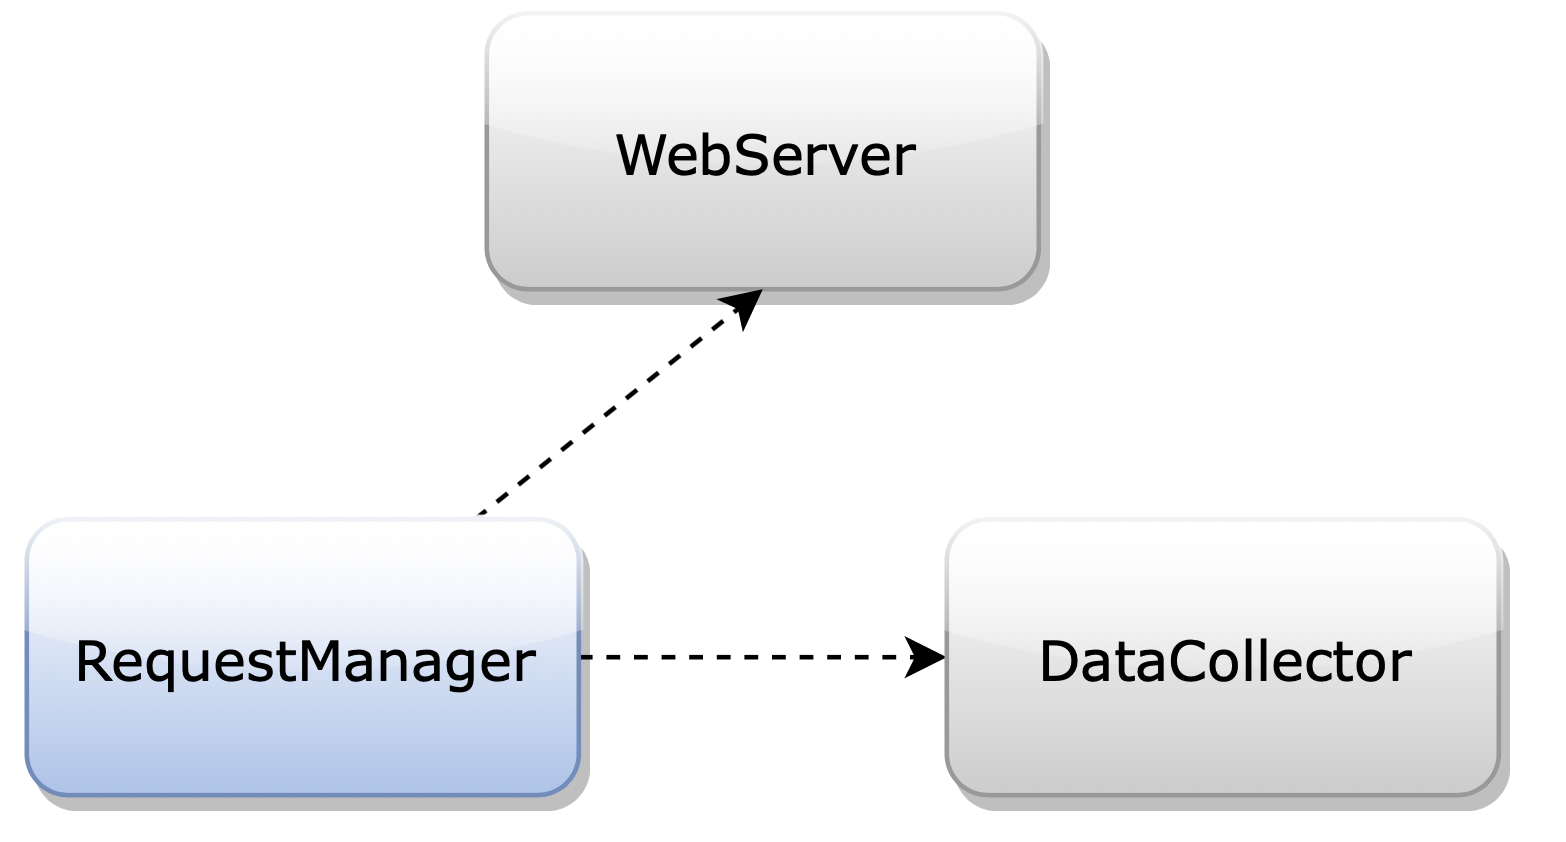
\includegraphics[scale=0.35]{Images/IntegrationPlanImages/fig1.png}
\caption{RequestManager Integration}
\end{figure}

\begin{figure}[H]
\centering
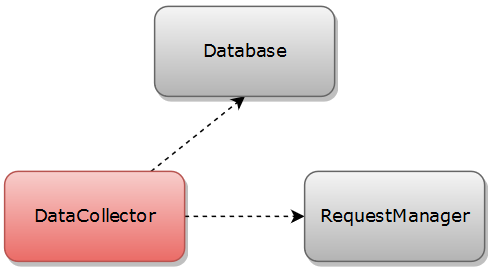
\includegraphics[scale=0.35]{Images/IntegrationPlanImages/fig2.png}
\caption{DataCollector Integration}
\end{figure}

\noindent
In the two diagrams above, RequestManager and DataCollector components are coupled twice, this means that the last component actually developed among them two will be integrated with the other one.

\begin{figure}[H]
\centering
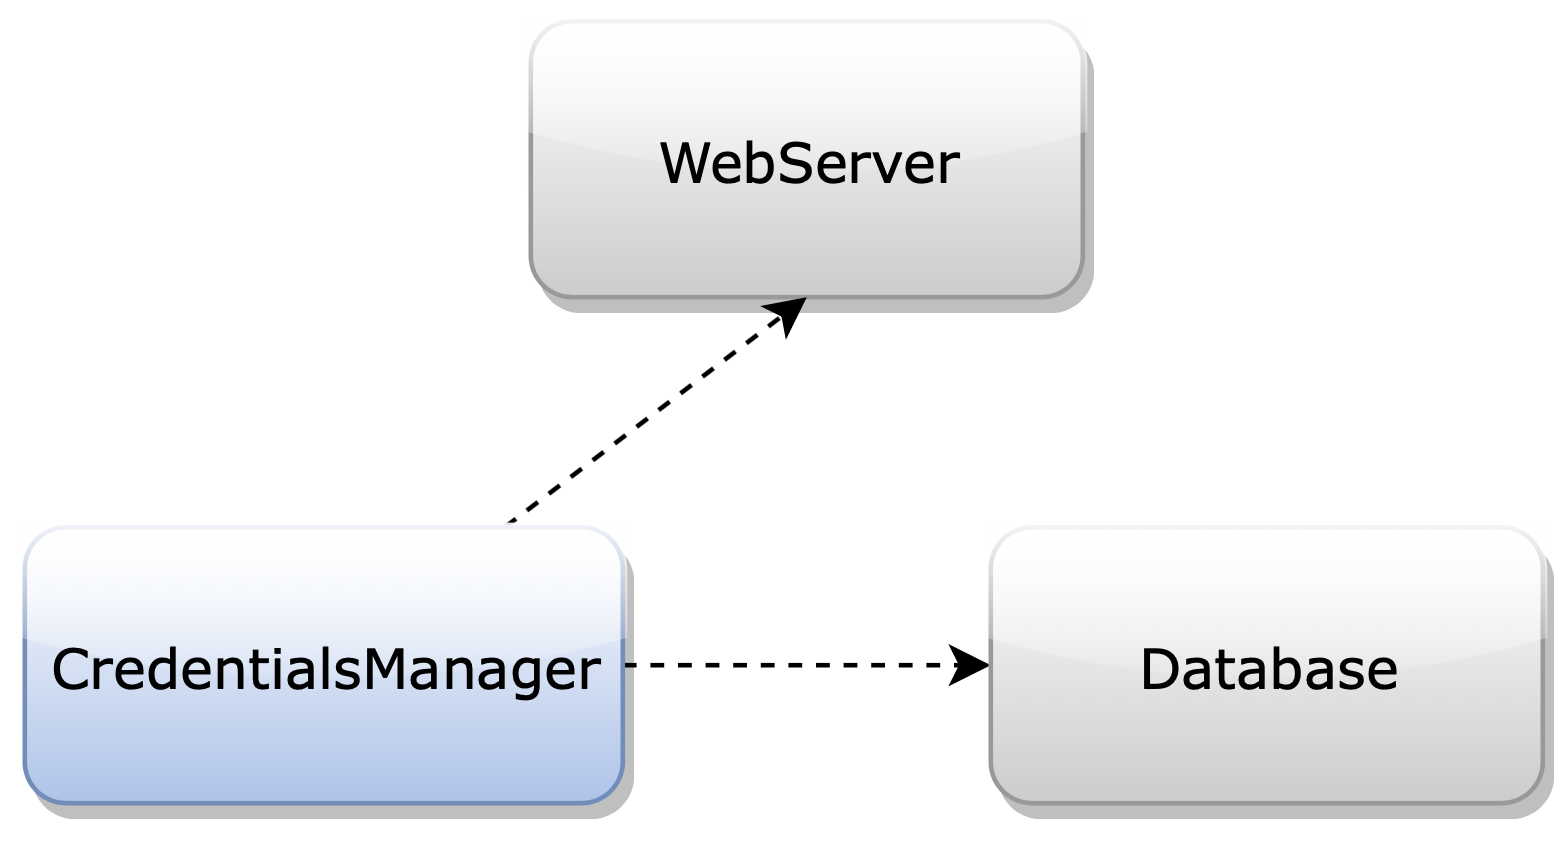
\includegraphics[scale=0.35]{Images/IntegrationPlanImages/fig3.png}
\caption{CredentialManager Integration}
\end{figure}

\begin{figure}[H]
\centering
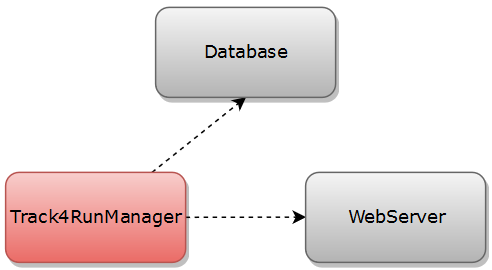
\includegraphics[scale=0.35]{Images/IntegrationPlanImages/fig4.png}
\caption{Track4RunManager Integration}
\end{figure}

\begin{figure}[H]
\begin{center}
        \begin{minipage}[c]{.40\textwidth}
	\centering
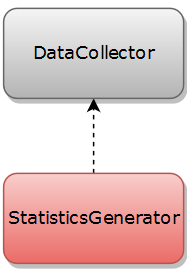
\includegraphics[scale=0.35]{Images/IntegrationPlanImages/fig5.png}
\caption{UserDataManager Integration}
        \end{minipage}%
        \hspace{10mm}%
        \begin{minipage}[c]{.40\textwidth}
	\centering
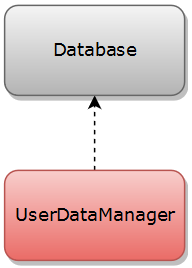
\includegraphics[scale=0.35]{Images/IntegrationPlanImages/fig6.png}
\caption{StatisticsGenerator Integration}
        \end{minipage}
      \end{center}
\end{figure}

\begin{figure}[H]
\begin{center}
        \begin{minipage}[c]{.40\textwidth}
	\centering
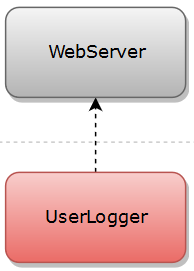
\includegraphics[scale=0.35]{Images/IntegrationPlanImages/fig7.png}
\caption{UserLogger Integration}
        \end{minipage}%
        \hspace{10mm}%
        \begin{minipage}[c]{.40\textwidth}
	\centering
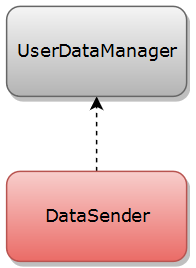
\includegraphics[scale=0.35]{Images/IntegrationPlanImages/fig8.png}
\caption{DataSender Integration}
        \end{minipage}
      \end{center}
\end{figure}

\begin{figure}[H]
\begin{center}
        \begin{minipage}[c]{.40\textwidth}
	\centering
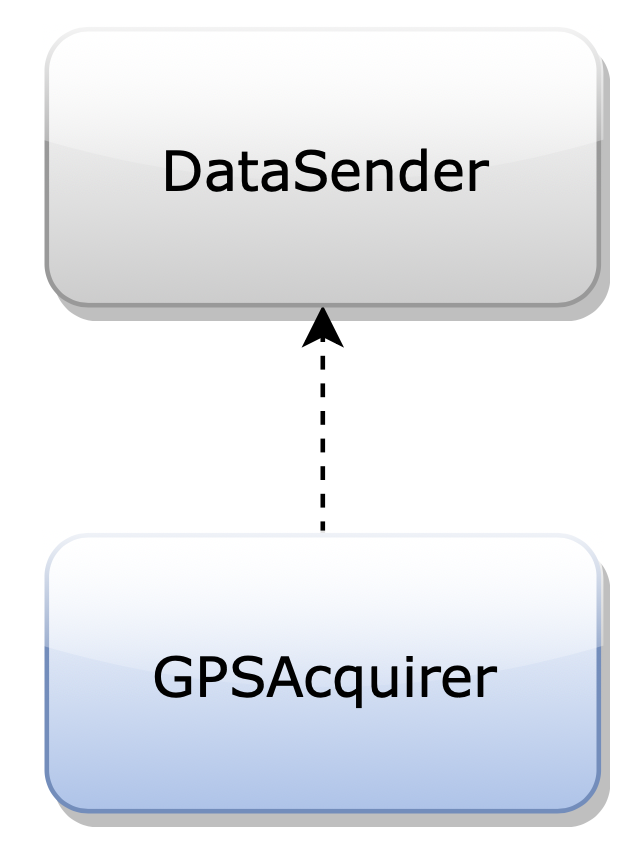
\includegraphics[scale=0.35]{Images/IntegrationPlanImages/fig9.png}
\caption{GPSAcquirer Integration}
        \end{minipage}%
        \hspace{10mm}%
        \begin{minipage}[c]{.40\textwidth}
	\centering
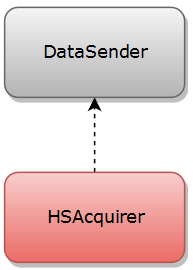
\includegraphics[scale=0.35]{Images/IntegrationPlanImages/fig10.png}
\caption{HSAcquirer Integration}
        \end{minipage}
      \end{center}
\end{figure}

\newpage

\begin{figure}[H]
\centering
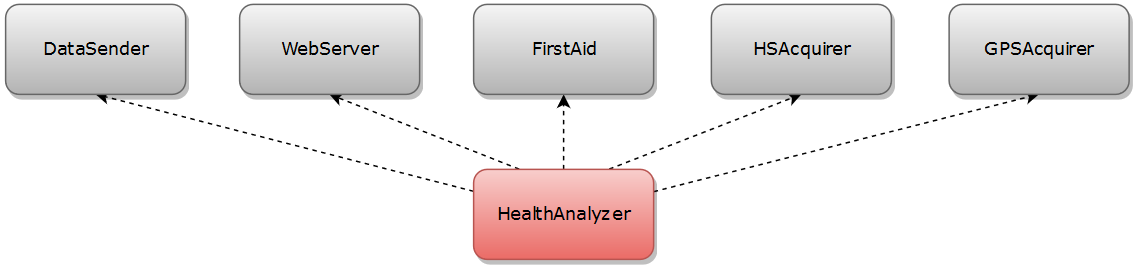
\includegraphics[scale=0.35]{Images/IntegrationPlanImages/fig11.png}
\caption{HealthAnalyzer Integration}
\vspace{0.8cm}
\end{figure}
\bigbreak
\begin{figure}[H]
\begin{center}
        \begin{minipage}[c]{.40\textwidth}
	\centering
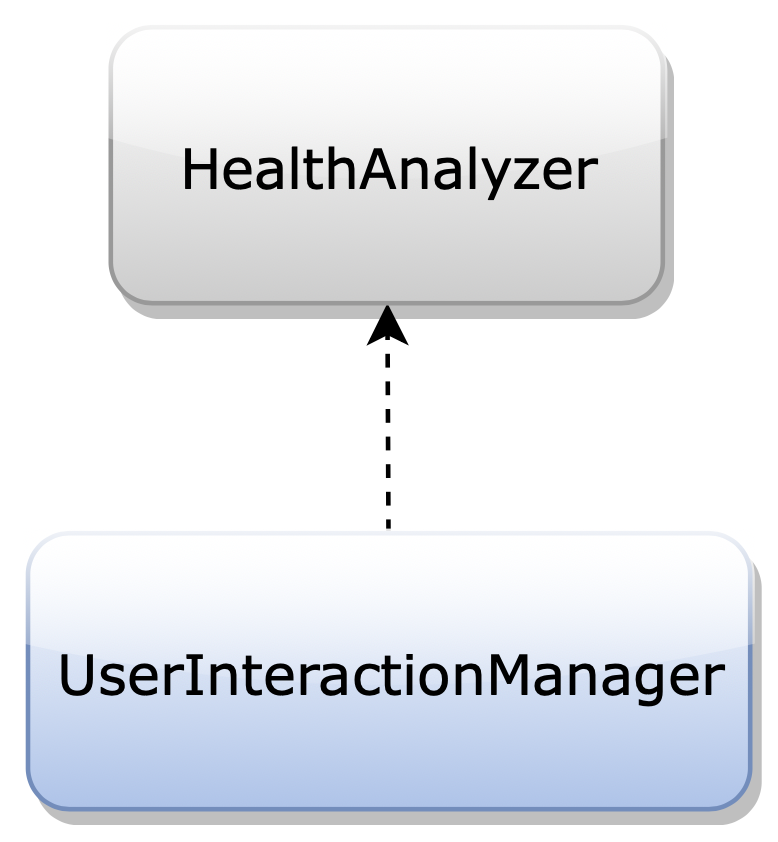
\includegraphics[scale=0.35,valign=t]{Images/IntegrationPlanImages/fig12.png}
\caption{UserInterfaceManager Integration}
        \end{minipage}%
        \hspace{10mm}%
        \begin{minipage}[c]{.40\textwidth}
	\centering
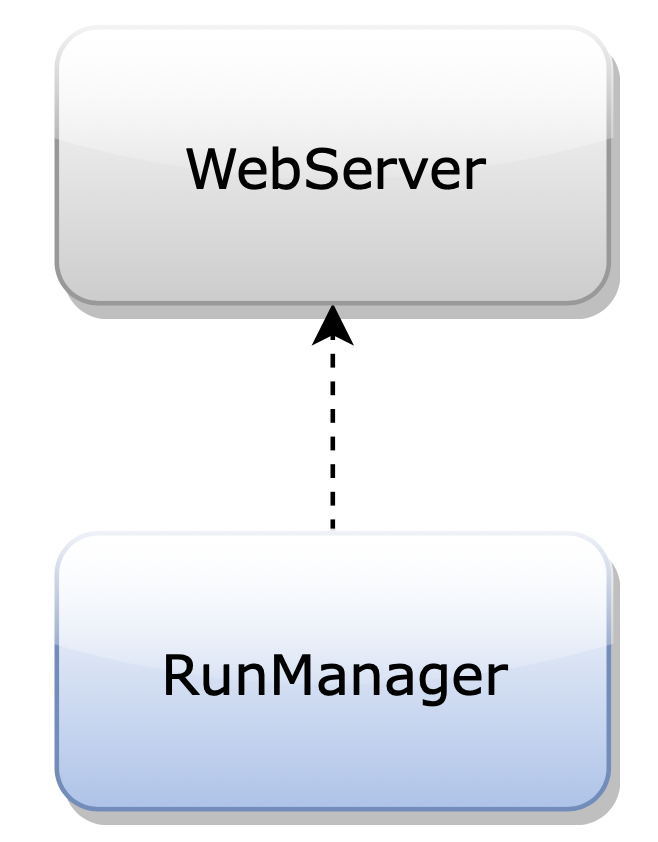
\includegraphics[scale=0.35,valign=t]{Images/IntegrationPlanImages/fig13.png}
\vspace{0.3cm}
\caption{RunManager Integration}
        \end{minipage}
      \end{center}
      \vspace{0.8cm}
\end{figure}

\begin{figure}[H]
\centering
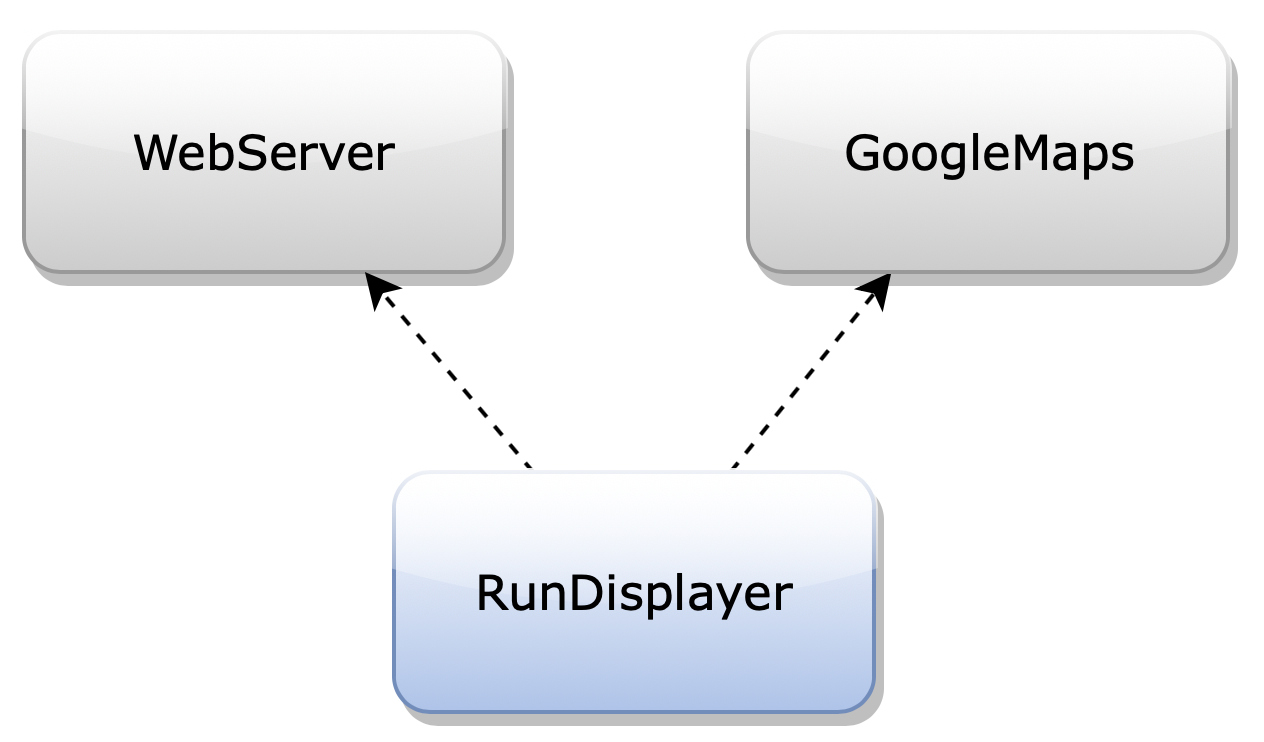
\includegraphics[scale=0.42]{Images/IntegrationPlanImages/fig14.png}
\caption{RunDisplayer Integration}
\end{figure}

\newpage
\subsubsection{Third Party Request Integration}
In the following two figures, the integration including more than two components at the same time are shown. More precisely, they explain the order in which components are integrated together in order to test the complete functionality of third parties' requests. As we stated before we adopted  an \textit{Incremental Integration and Testing} approach and, therefore, we add to the integration one component at a time until we got the full chain of components which should perform the complete functionality.
\begin{figure}[H]
\centering
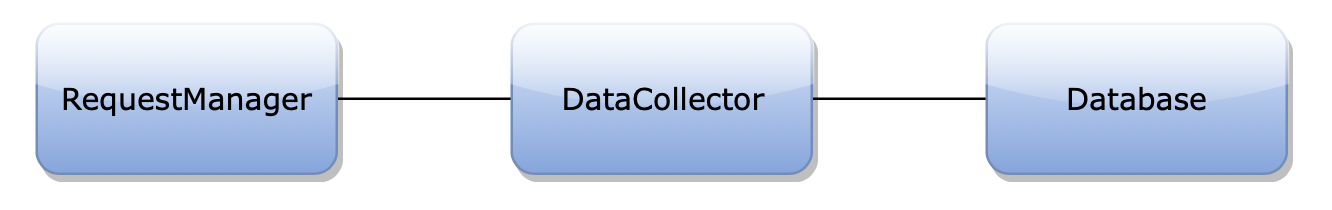
\includegraphics[scale=0.65]{Images/IntegrationPlanImages/fig15.png}
\caption{ThirdPartyRequest semi-chain integration}
\end{figure}

\begin{figure}[H]
\centering
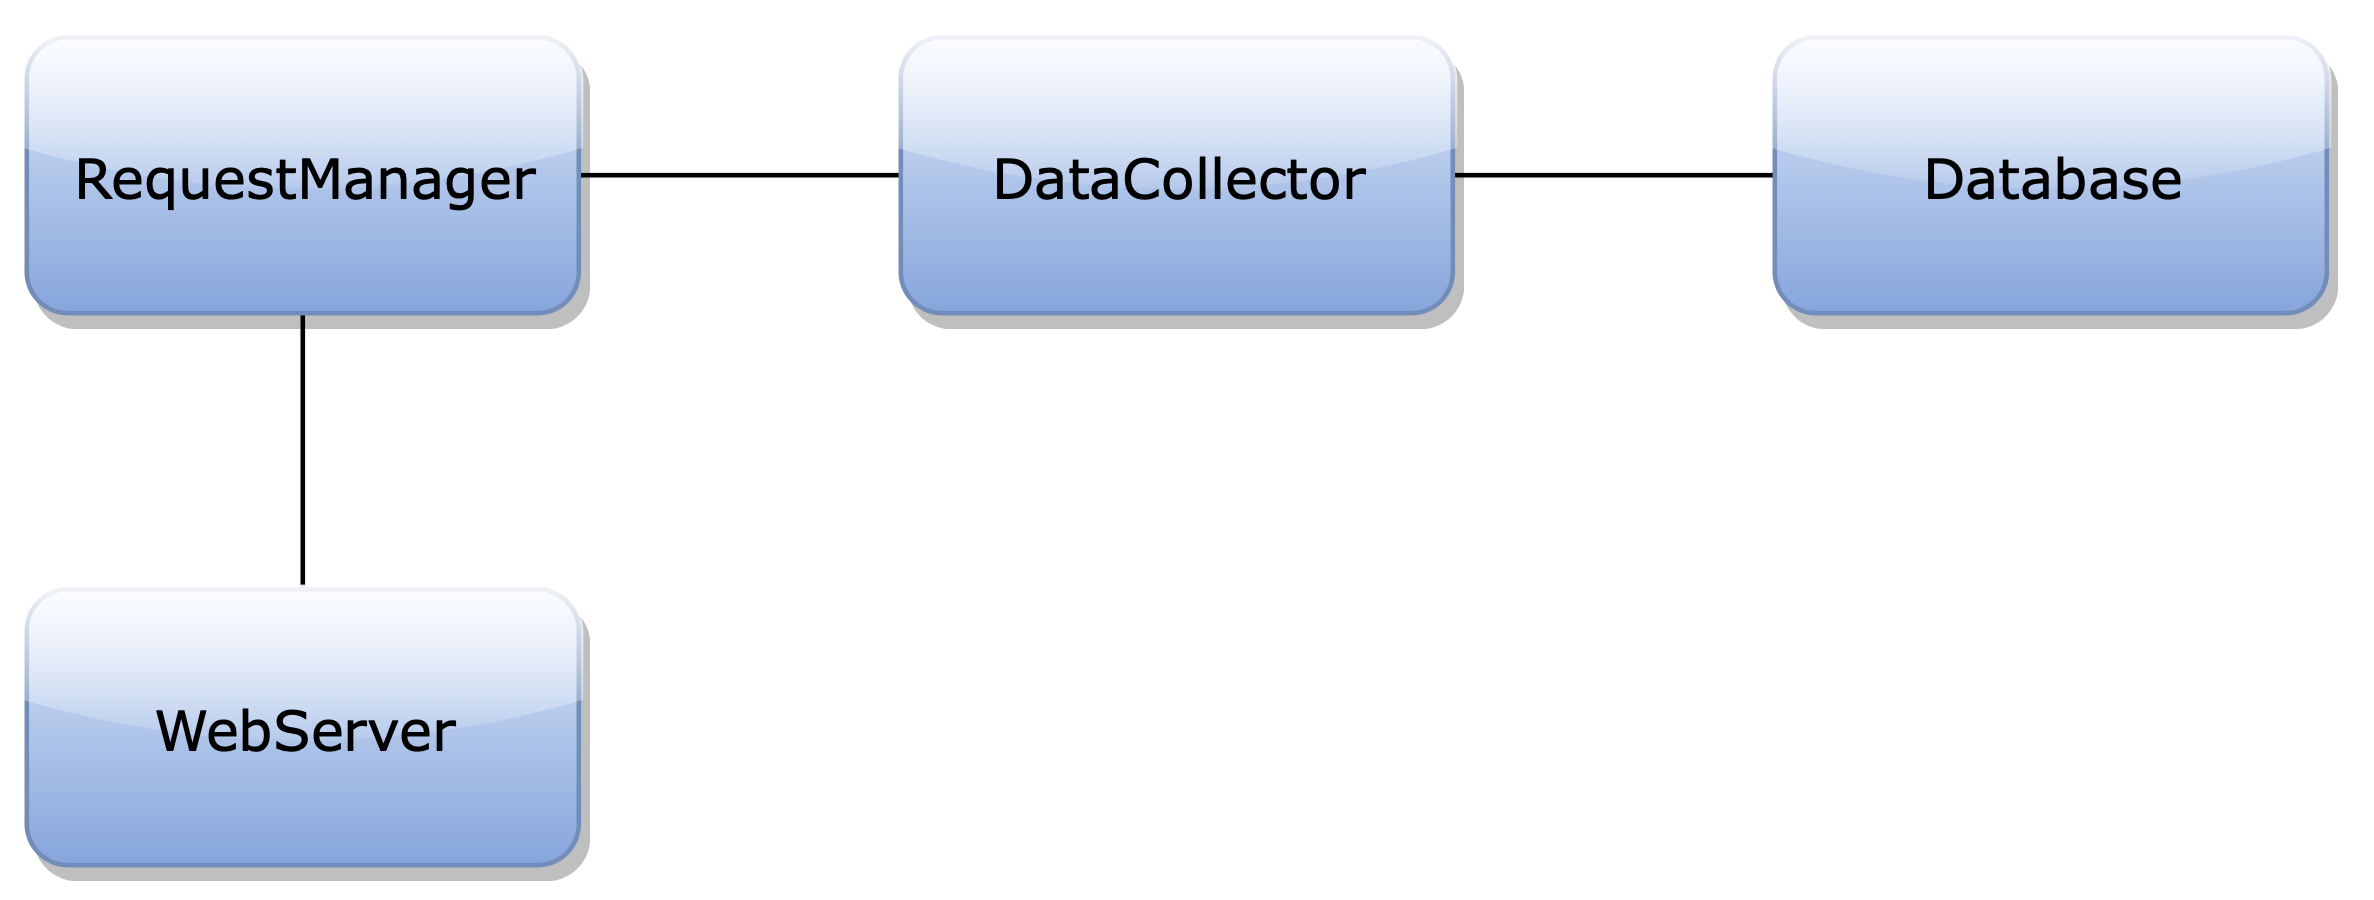
\includegraphics[scale=0.35]{Images/IntegrationPlanImages/fig16.png}
\caption{ThirdPartyRequest full-chain integration}
\end{figure}

\subsubsection{Run Event Storing Integration}
The next two figures shows integration including more than two components at the same time. More precisely, they explain the order in which components are integrated together in order to test the complete functionality of storing into the Database all the information regarding run events. 
\begin{figure}[H]
\centering
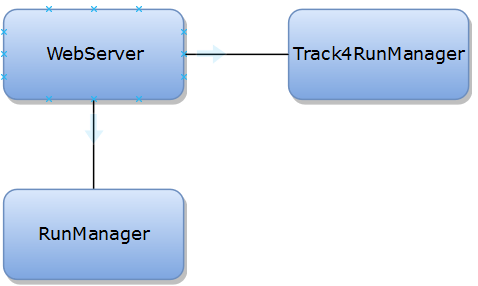
\includegraphics[scale=0.65]{Images/IntegrationPlanImages/fig17.png}
\caption{Run event storing semi-chain integration}
\end{figure}

\begin{figure}[H]
\centering
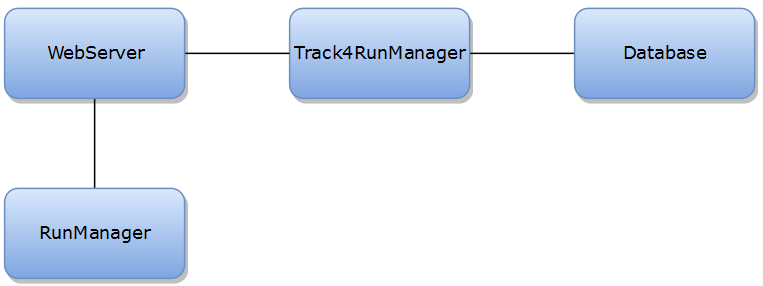
\includegraphics[scale=0.35]{Images/IntegrationPlanImages/fig18.png}
\caption{Run event storing full-chain integration}
\end{figure}


\subsection{System Testing}
Once the system is integrated completely and once it has an acceptable performance it will be tested as a whole. This due to the fact that in the future the system could possibly be subject to heavy workloads. System Testing will identify the following problems:

\begin{itemize}
\item Inefficient algorithms: it's really important to have efficient algorithms implemented in the system, especially for the RequestManager, that manages the requests deciding which one is more urgent, and especially for the HealthAnalyzer which needs to have very small reaction time in order to call the ambulance as soon as possible.
\item Query optimization problems: taking into account that the system's functionality heavily relies on queries, testing on DB query optimization is for sure a good test to implement.
\item Hardware issues: taking into account that the system relies on some piece of hardware that our system cannot directly test, such as the GPS and HS hardware retrievers, it can be important to check if the data retrieved are subjected to relevant noise.
\item Network issues: it's really important to check how much request load the Web Server can withstand and if necessary to expand the connection broadband.
\end{itemize}

\noindent
More precisely two types of System Testing will be done:
\medbreak
\noindent
\textbf{Load Testing  \begin{large} $\rightarrow$ \end{large}} increasing the load of the system for a long period of time in order to find and solve memory leaks, buffer overflows, bad memory management and also identify upper limits of components.
\medbreak
\noindent
\textbf{Stress Testing  \begin{large} $\rightarrow$ \end{large}} trying to break the system by overwhelming its resources or by taking resources away from it will make sure that the system recovers gracefully after failure, this is very important for our system especially for AutomatedSOS components which are in charge of giving real time assistance to users that suffer from health issues.



